\documentclass[12pt, oneside]{article}

\usepackage{texmf/preamble}
\usepackage{texmf/macros}
\usepackage{texmf/wordcount}

\graphicspath{{./assets/}}
\addglobalbib{sources.bib}

% =================================================================
% Content
% =================================================================


\begin{document} % BEGIN
\pagestyle{frontmatter}

\begin{titlepage}
    \large

    \begin{center}

        \vspace*{2cm}

        {\bfseries
            IB Math Analysis and Approaches (HL) \\
            Extended Essay\\
            May 2024 Session}\\

        \vspace*{\fill}

        \rule{\linewidth}{1.5pt} \\ [0.5cm]
        {\LARGE \bfseries The Mathematics Techniques of Camera Calibration}
        \rule{\linewidth}{0.5pt} \\

        \vspace*{\fill}

        \textbf{Research Question:} What are the various strategies and mathematical techniques employed in camera calibration to develop precise and accurate camera models?\\ [1cm]

        \textbf{Word Count:} \wordcount words

        \vspace*{2cm}

    \end{center}

\end{titlepage}

% =================================================================
\pagenumbering{roman}
\tableofcontents
% =================================================================
\clearpage
\pagestyle{mainmatter}
\pagenumbering{arabic}
\setcounter{page}{1}

\section{Introduction}

3D reconstruction from multiple images is the process of generating an accurate 3D model of a physical object from its 2D images. The process employs techniques from the broader science of photogrammetry, which is concerned with obtaining precise measurements of 3-dimensional physical objects from photographic images. The use of photogrammetry as a method of 3D reconstruction was first employed by Prussian architect Albrecht Meydenbauer in the 1860s, who created some of the earliest topographic plans and elevations drawings realized using photogrammetric techniques \autocite{ices2017}. Today, photogrammetry has applications in a wide variety of fields, including but not limited to: architecture, engineering, forensics, medicine, and geology.

\subsection{Overview of 3D Reconstruction}



The task of generating an accurate 3D model from various 2D images is a multi-step process, and consists of:




and they mainly fall into two main categories. The first method is based on the cross-referencing of keypoints between the images. Computer algorithms such as SIFT (Scale Invariant Feature Transform) and SURF (Speeded-Up Robust Features)

projective geometry to triangulate the position of keypoints of the objects. These keypoints are cross-referenced between the images either by hand or using a computer algorithm, and then


Camera calibration is a important








\section{Approach} 

There are many techniques one could take to calibrate a camera, 




\subsection{Camera Model} \label{sec:camera_model}

A camera model is a projection model which approximates the function of a camera by describing a mathematical relationship between points in 3D space and its projection onto the sensor grid of the camera. In order to construct such a model, we must first understand the general workings of a camera.

The modern lens camera is highly sophisticated, built with an array of complex mechanisms and a wide range of features such as zoom and autofocus. However, we only need to focus on its three principal elements critical to image projection: the lens, the aperture, and the sensor grid (CCD). 

\begin{itemize}[leftmargin=!, itemindent=-5ex]
    \item \textbf{Lens} -- Focuses incoming light rays and projects it onto the sensor grid. Modern cameras have compound lenses (lenses made up of several lens elements) in order to minimize undesired effects such as aberration, blurriness, and distortion. 
    \item \textbf{Aperture} -- Controls the amount of light that reaches the sensor. By adjusting the aperture size, the exposure and depth of field can be modified.
    \item \textbf{Sensor Grid} -- Captures incoming light rays and converts this information into pixels on an image. 
\end{itemize}

\begin{figure}[H]
    \centering
    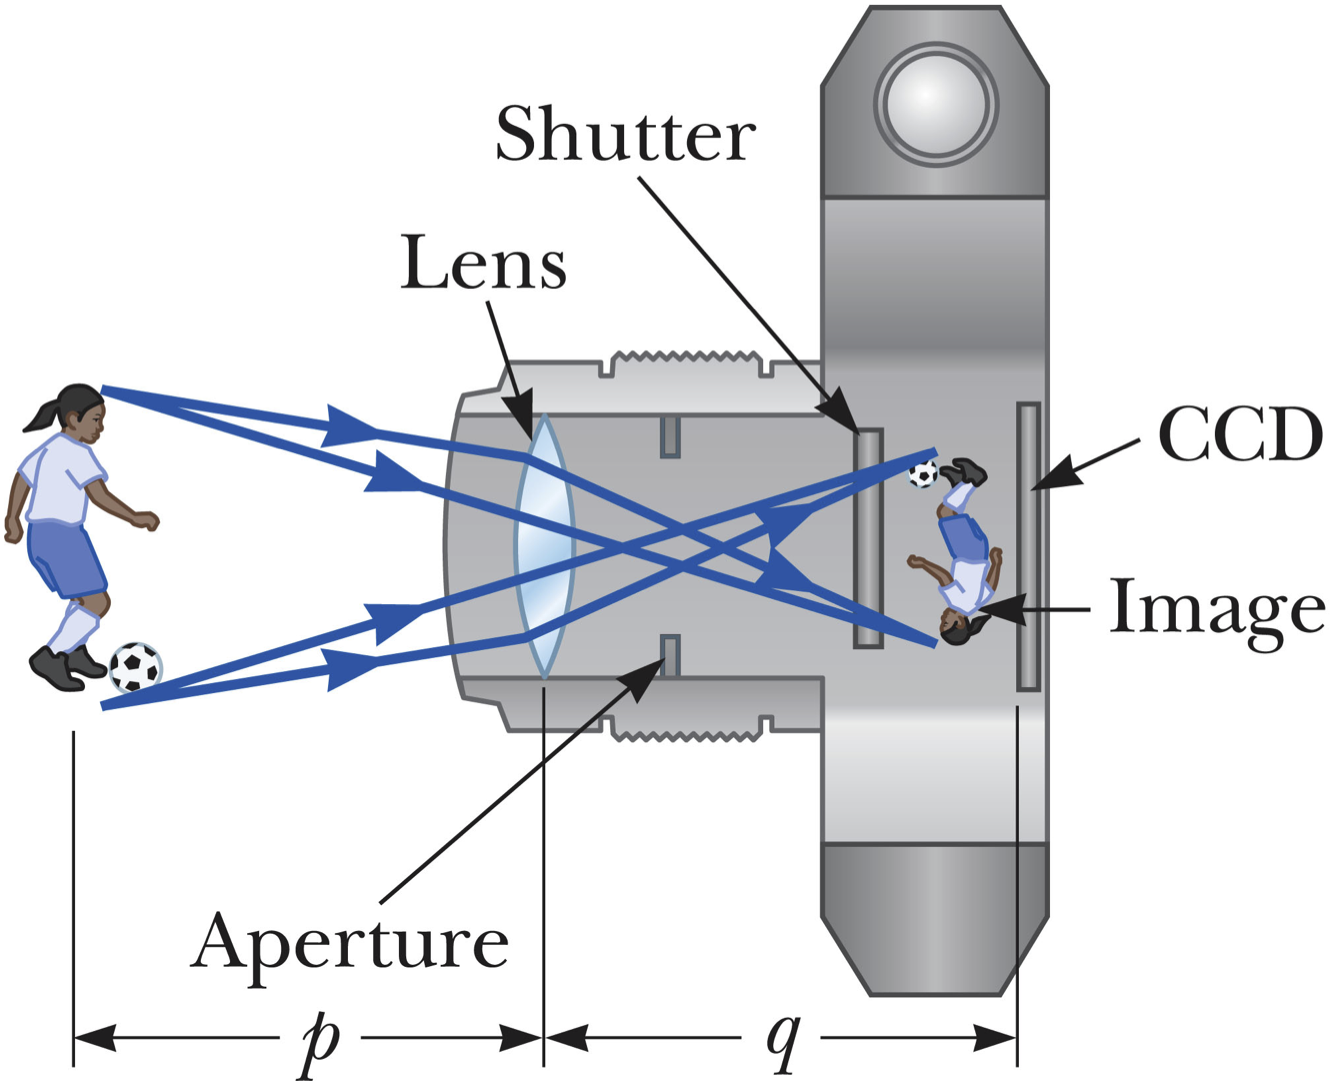
\includegraphics[width=0.5\textwidth]{images/lens_camera}
    \caption{Lens camera. Adapted from \cite{coltonPhysics1232012}} \label{fig:lens_camera}
\end{figure}

However, it is impossible to construct a model which is both simple and exact for the lens cameras, as the behavior of lenses are very complex. As such, it is mathematically convenient to approximate the camera as a pinhole camera. In doing so, we ignore lens distortion, but it distills the behavior of a camera to its most fundamental and essential dynamics: the projection of points in 3D space onto the flat 2D image plane. 

\subsubsection{Pinhole Camera Model}

A pinhole camera is a simple camera without a lens. It instead relies on the use of a tiny hole as the aperture of the camera, and light rays pass through the hole, projecting an inverted image onto the image plane. The pinhole camera model is based on the pinhole camera, however it goes further by making the assumption that the aperture is infinitely small. This means that any incoming light ray would only travel in straight lines, going through the pinhole mapping to one singular point on the image plane. 

\begin{figure}[H]
    \centering
    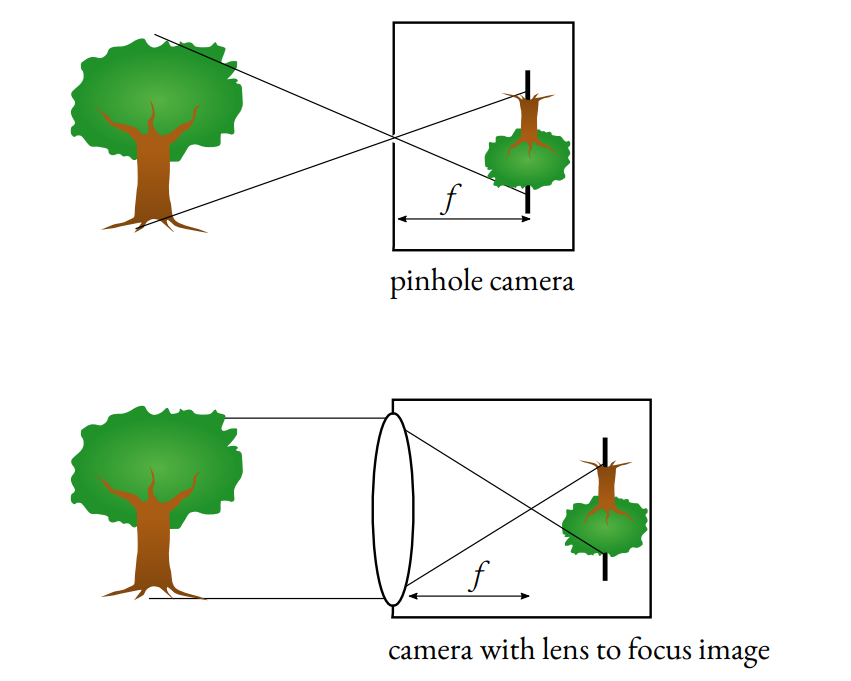
\includegraphics[width=0.7\textwidth]{images/pinhole_vs_lens}
    \caption{Difference between a pinhole camera and a lens camera. Adapted from \cite{leCameraModel2018}}
\end{figure}

If necessary, one could reintroduce distortion and shear terms in order to minimize the error, but this is often not needed for low to medium precision applications, as the distortion of modern lenses are already minimal. As such, its ease of use has led it to become one of the most frequently employed camera models in the field of camera calibration. 

\subsection{Calibration Object}

The calibration object is an object with known dimensions and features which is often used in camera calibration to 


Calibration objects can be constructed in many ways, and they can be separated into different categories based the dimension of the calibration object \footcite{zhangCameraCalibration2007}.

\begin{itemize}[leftmargin=!, itemindent=-4ex]
    \item \textbf{3D object based calibration} -- Performed by using a calibration object whose geometry is known to very high precision. Typically, the calibration object consists of 2 or 3 orthogonal planes, although a plane whose precise translation is known may also be used, which also yields 3D reference points \footcite{zhangCameraCalibration2007}. Using 3D objects is typically preferred, as it yields the highest accuracy \footcite{zhangCameraCalibration2007}, and the mathematics required is also the least. 
    \item \textbf{2D plane-based calibration} -- The most common technique is known as Zhang's method, and it requires a planar object (often a checkerboard pattern), and various pictures of this plane are taken at different orientations \footcite{zhangFlexibleNew2000}. Knowledge of the translation of the plane is not necessary. Due to its easier setup and good accuracy, it is the best choice in most situations. In fact, the most commonly used camera vision programming library, \texttt{OpenCV}, is geared towards this type of calibration. 
    \item \textbf{1D line-based calibration} -- Typically requires analyzing more than three photographs with straight lines which are not parallel with each other \footcite{chuLineBasedCamera2005}. 
\end{itemize}

One can also calibrate cameras without a calibration object, using featuring tracking of objects in the scene to estimate camera parameters. This process is often referred to as self-calibration or auto-calibration. However, this is less preferable, as it involves a lot of estimation of parameters, which not only means that it is a more mathematically complex problem, it may not be able to achieve the accuracy of calibration using known calibration patterns \footcite{zhangCameraCalibration2007}. As such, it is typically the only chosen when pre-calibration is impossible. 

For this paper, I will focus on calibration using a 3D calibration object, because the mathematics behind it is simpler, and many of the techniques used in 3D-based calibration are 

\section{Prerequisites}

Given the that this paper utilizes mathematical concepts beyond the scope of the IB Mathematics Analysis and Approaches HL curriculum, it is imperative that some notation and important ideas are introduced prior.

\subsection{Notation}
\noindent\textbf{Vectors and Matrices.} In this paper, lowercase letters are used to denote vectors, whereas capital letters are used for matrices. Depending on the context, vectors can also be attached with diacritics:
\begin{itemize}[leftmargin=!, itemindent=-4ex]
    \item \textbf{$\vec{v}$} -- a letter with an arrow above it denotes a positional vector or translational vector dealing with the transformation of points in space.
    \item \textbf{$\widetilde{v}$} -- a letter with a tilde above it denotes a vector represented in homogenous coordinates. This idea is explained in section \ref{sec:homogenous}.
    \item \textbf{$v$} -- when explicitly stated, a letter without diacritics can also denote a vector if it does not fall into the categories listed above. 
\end{itemize}

\noindent\textbf{Transpose of Vectors and Matrices.} The transpose of a vector or a matrix is an operation whereby the rows and columns of the vector or matrix are inverted, and this is denoted using the notation $v^\T$ or $M^\T$. For example:
\[
    \begin{bmatrix}
        a & b \\
        c & d
    \end{bmatrix}^\T
    =
    \begin{bmatrix}
        a & c \\
        b & d
    \end{bmatrix}
\]

\subsection{Homogenous Coordinates} \label{sec:homogenous}

While Euclidean space describes 2D and 3D space well, they are not sufficient in describing perspective projections, as it is unable to fully the capture the relationships inherent in projective projections and affine transformations, both of which are core concepts in this paper. 

Homogenous coordinates forms the basis of projective geometry, because it unifies the treatment of common graphical transformations such as rotation and translations \footcite[][1]{bloomenthalHomogeneousCoordinates1994}. 

Given a point in with $\Real^n$ coordinates $(a_1, a_2, \cdots, a_n)$

When



Given the vector $[\,x, y\,]^\T \in \Real^2$, we can express it in terms of homogenous coordinates: 
\begin{equation}
    \begin{bmatrix}
        x \\ y
    \end{bmatrix}
\end{equation}

\begin{figure}[H]
    \centering
    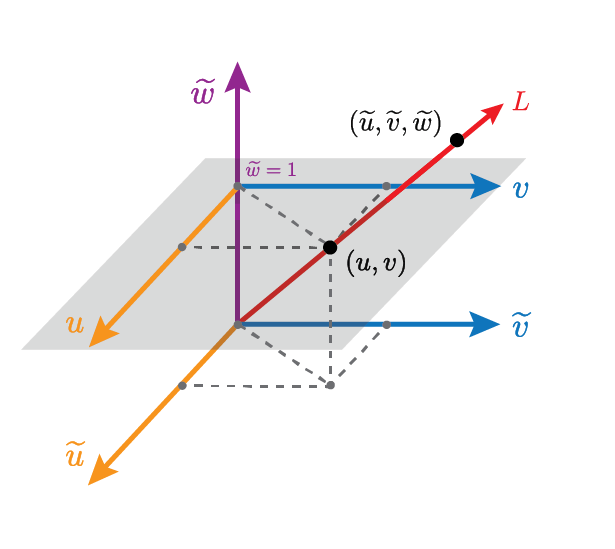
\includegraphics[width=0.6\textwidth]{figures/homogenous}
    \caption{Homogenous coordinate system.}
\end{figure}

In other words, with homogenous coordinates, we interpret our \emph{Euclidean} space as an \emph{affine} space

\section{Constructing the Pinhole Camera Model}

For our camera model, we will introduce 4 different frames of reference, all of which :
\begin{itemize}[leftmargin=!, itemindent=-4ex]
    \item\textbf{World Coordinate Frame ($\boldsymbol{\mathcal{W}}$)}. Represents the 3D space of the scene being photographed, with respect to an origin which may be arbitrary and depends on the conventions chosen. Objects that are in the scene are defined with respect to this coordinate frame. 
    \item\textbf{Camera Coordinate Frame ($\boldsymbol{\mathcal{C}}$)}. Represents the 3D space of the scene being photographed, but with respect to the pinhole (aperture) of the camera. 
    \item\textbf{Image Coordinate Frame ($\boldsymbol{\Pi}$)}. 2D plane representing the image sensor plane of the camera. The origin is the principle point of the image sensor, where the optical axis intersects the image plane. 
    \item\textbf{Pixel Coordinate Frame}. 2D plane representing the position of pixels on the image sensor. The Discrete version of the image coordinate frame, where c
\end{itemize}

The optical axis of a camera is an imaginary line which passes through the center of the aperture of the camera. 



\begin{figure}[H]
    \centering
    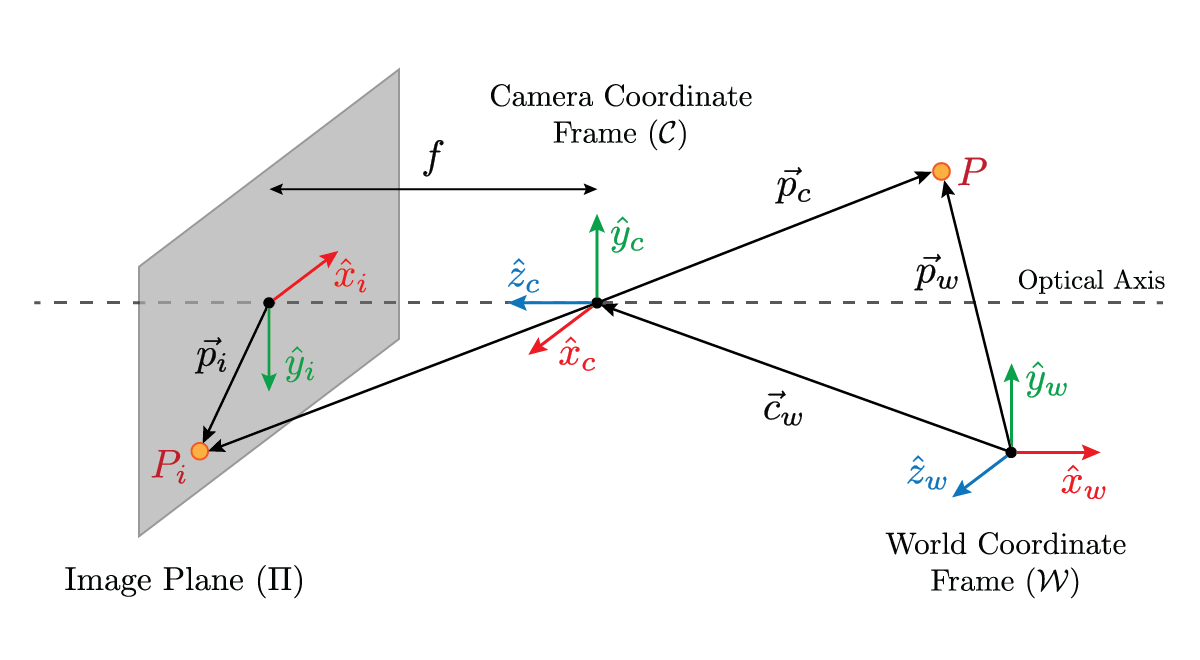
\includegraphics[width=0.9\textwidth]{figures/imaging_model}
    \caption{Pinhole camera model.}
\end{figure}

\begin{figure}[H]
    \centering
    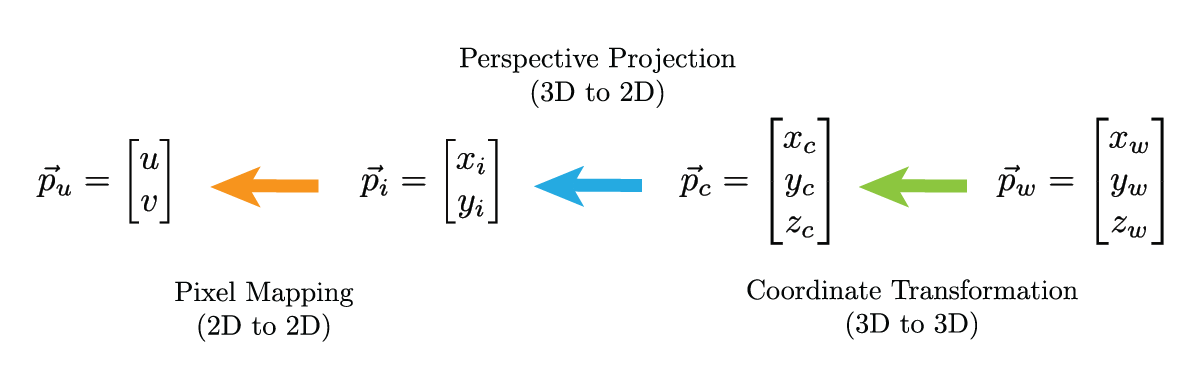
\includegraphics[width=0.9\textwidth]{figures/coord_conversions}
    \caption{Coordinate transformations.}
\end{figure}


\subsection{Extrinsic Parameters} \label{sec:extrinsics}

First, we need to establish the relationship between position of a point in the camera coordinate frame $\mathcal{C}$ to their position in the world coordinate frame $\mathcal{W}$. To do so, we find the extrinsic matrix $T$, which relates the positional vector $\vec{p}_w$ of point $P$, to its positional vector.
\begin{equation} \label{eq:pc}
    \vec{p}_c = T\vec{p}_w
\end{equation}

\begin{figure}[H]
    \centering
    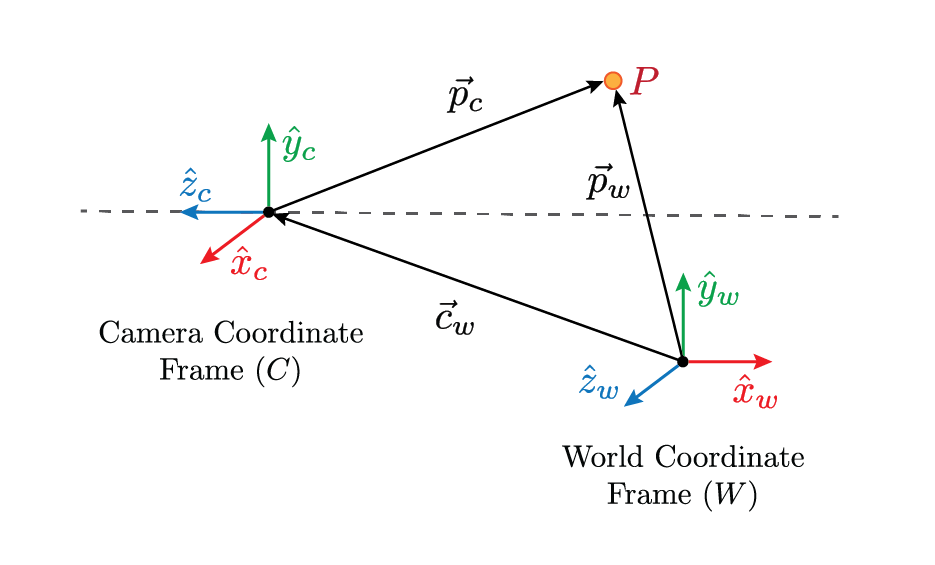
\includegraphics[width=0.9\textwidth]{figures/coord_transform}
    \caption{Coordinate transformation from the world coordinate frame to the camera frame.}
\end{figure}


For the extrinsic parameters of the camera, we have the position $\vec{c}_w$ of the camera in world coordinates and orientation $R$ of the camera. The orientation, $R$, is a 3x3 rotational matrix:

\begin{equation}
    R =
    \begin{bmatrix}
        r_{11} & r_{12} & r_{13} \\
        r_{21} & r_{22} & r_{23} \\
        r_{31} & r_{32} & r_{33}
    \end{bmatrix}
\end{equation}

\noindent where:
\begin{itemize}
    \item Row 1: Direction of $\hat{x}_c$ in world coordinate frame.
    \item Row 2: Direction of $\hat{y}_c$ in world coordinate frame.
    \item Row 3: Direction of $\hat{z}_c$ in world coordinate frame.
\end{itemize}

\noindent

\begin{subequations}
    \begin{align}
        \vec{p}_c & = R(\vec{p}_w-\vec{c}_w) \\
                  & = R\vec{p}_w -R\vec{c}_w
    \end{align}
\end{subequations}



\begin{gather}
    \vec{p}_c = R\vec{p}_w + \vec{t} \\
    \begin{bmatrix}
        x_c \\ y_c \\ z_c
    \end{bmatrix}
    =
    \underbrace{
        \begin{bmatrix}
            r_{11} & r_{12} & r_{13} \\
            r_{21} & r_{22} & r_{23} \\
            r_{31} & r_{32} & r_{33}
        \end{bmatrix}
    }_{\mathlarger{R}}
    \begin{bmatrix}
        x_w \\ y_w \\ z_w
    \end{bmatrix}
    +
    \underbrace{
        \begin{bmatrix}
            t_x \\ t_y \\ t_z
        \end{bmatrix}
    }_{\mathlarger{\vec{t}}}
\end{gather}


\begin{equation}
    \begin{bmatrix}
        x_c \\ y_c \\ z_c 
    \end{bmatrix}
    =
    \underbrace{
        \begin{bmatrix}
            r_{11} & r_{12} & r_{13} & t_x \\
            r_{21} & r_{22} & r_{23} & t_y \\
            r_{31} & r_{32} & r_{33} & t_z \\
        \end{bmatrix}
    }_{\mathlarger{T}}
    \begin{bmatrix}
        x_w \\ y_w \\ z_w \\ 1
    \end{bmatrix}
\end{equation}

\begin{equation}
    T = \left[\,R\,\vert\,\vec{t}\:\right]
\end{equation}


\subsection{Intrinsic Parameters} \label{sec:intrinsics}

Intrinsic parameters describe the internal characteristics of the camera. In other words, it dictates how in the 3D space are projected onto the image plane. We As such, our goal is to construct a calibration matrix, $K$, which relates the position of the point $P$ to its projection on the image plane. This can be expressed mathematically as follows:
\begin{equation} \label{eq:pi}
    \vec{p}_i =  K\vec{p}_c
\end{equation}
where $\vec{p}_i$ and $\vec{p}_c$ represents the position of the point $P$ on the image plane $\Pi$ and the camera frame $\mathcal{C}$ respectively.
\begin{figure}[H]
    \centering
    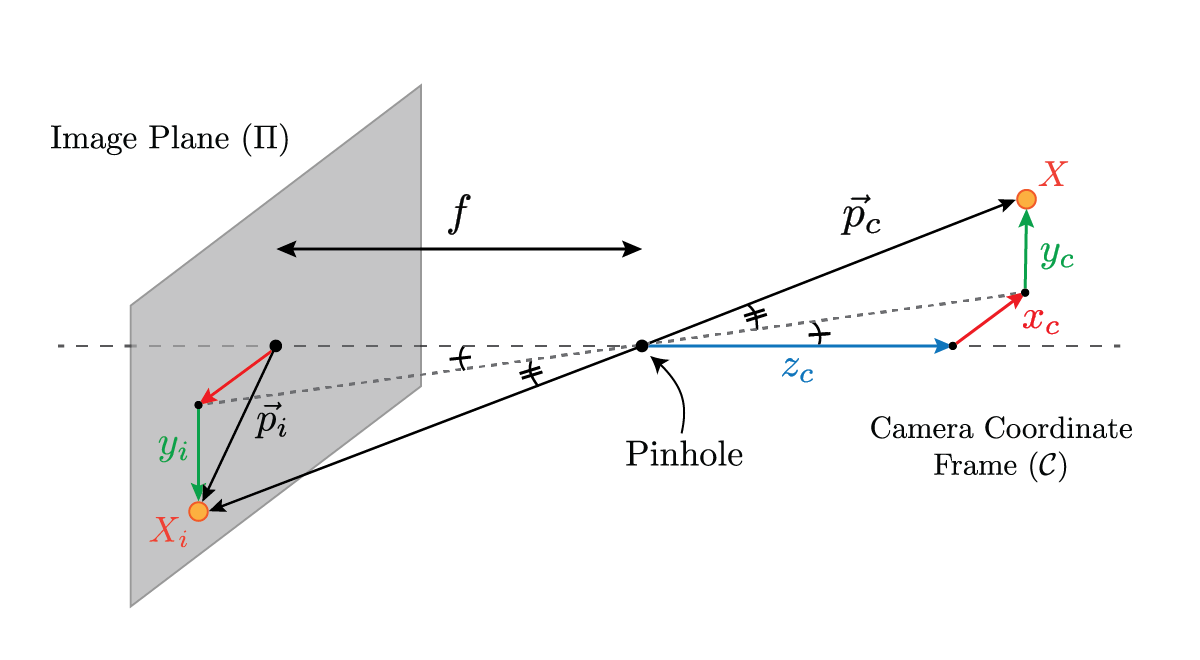
\includegraphics[width=0.9\textwidth]{figures/perspective_projection}
    \caption{Perspective projection of the point $P$ onto the image plane $\Pi$.}
\end{figure}
When a straight line is drawn from $P$ to its projection $P_i$ through the aperture, it intersects the optical axis. Deconstructing this intersection in the $x$ and $y$ direction, pairs of similar triangles are formed, which relates $x_i$ to $x_c$ and $y_i$ to $y_c$.
\begin{figure}[H]
    \centering
    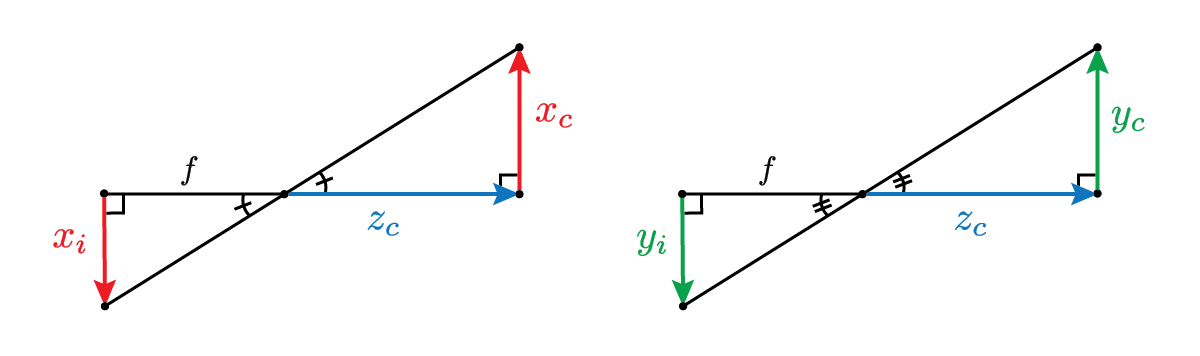
\includegraphics[width=\textwidth]{figures/similar_triangles}
    \caption{Similar triangles formed by perspective projection, which relate $x_i$ to $x_c$ and $y_i$ to $y_c$.} \label{fig:similar_triangles}
\end{figure}
\begin{subequations}
    \begin{gather}
        \frac{x_i}{f} = \frac{x_c}{z_c} \quad \Longrightarrow \quad x_i = f \frac{x_c}{z_c} \label{subeq:xi_result}\\
        \frac{y_i}{f} = \frac{y_c}{z_c} \quad \Longrightarrow \quad y_i = f \frac{y_c}{z_c} \label{subeq:yi_result}
    \end{gather}
\end{subequations}
Once the coordinates of the point projection, $(x_i, y_i)$, is known, we then need to convert it to actual pixel position of the point on the image, $(u, v)$. Pixel coordinates are measured in pixels, from the left-hand corner of the image. This is the convention that is typically followed in computer graphics. As such, there will be an offset in pixels, $(c_x, c_y)$, which represents the optical center of the image (i.e. the point at which the optical axis intersects the image plane). Additionally, the relationship between $(x_i, y_i)$ and $(u, v)$ is proportional, but they scale at different rates, as $(x_i, y_i)$ can be measured using any unit measurement, and can have negative and decimal values. On the other hand, $(u,v)$ are measured in discrete pixel value, which can different sizes depending on the camera used. As such, we define scaling factors, $m_x$ and $m_y$, be scaling factors which represent the pixel density of the image sensor in the $x$ and $y$ axes of the image sensor plane respectively. 
\begin{figure}[H]
    \centering
    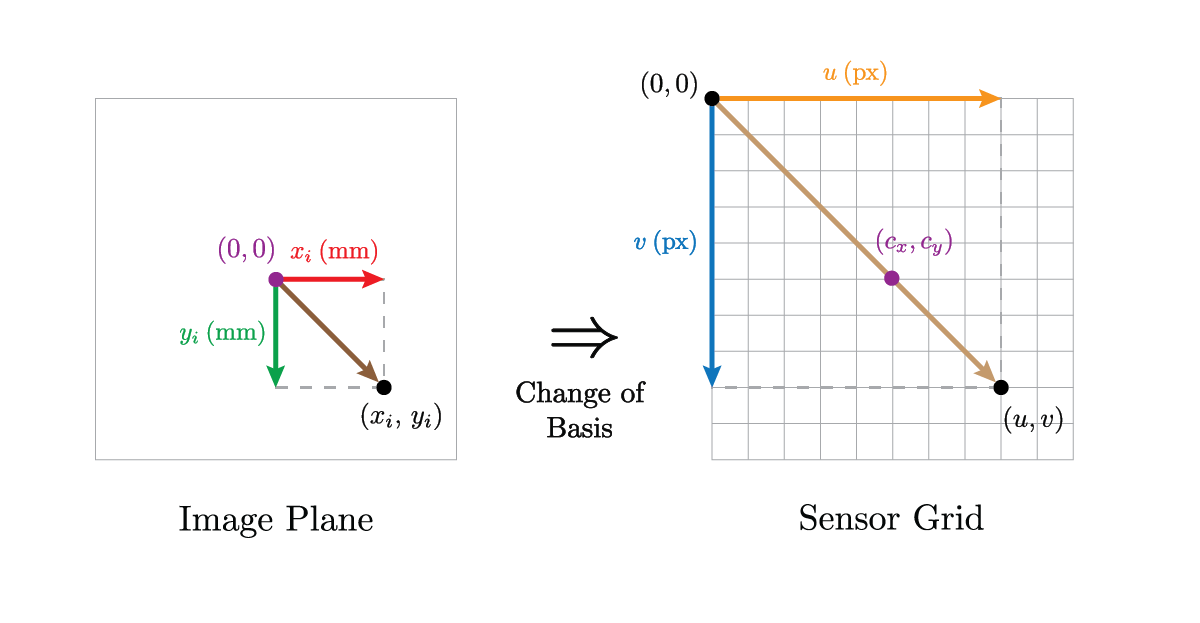
\includegraphics[width=\textwidth]{figures/sensor_grid}
    \caption{Conversion from image plane coordinates to sensor grid coordinates}
\end{figure}
Putting all the ideas above together, we can construct a set of linear parametric equations relating the pixel coordinates to their image coordinates thus: 
\begin{align*}
    u = m_x x_i + c_x \\
    v = m_y y_i + c_y
\end{align*}
where $u,v \in \Integer^+_{\,*}$. Replacing $x_i$ and $y_i$ for the result we obtained from equations \ref{subeq:xi_result} and \ref{subeq:yi_result}, we get:
\begin{align*}
    u = m_x f \frac{x_c}{z_c} + c_x \\
    v = m_y f \frac{y_c}{z_c} + c_y
\end{align*}
This gives us a direct relationship between camera coordinates and their corresponding pixel coordinates. Since $m_x$, $m_y$, and $f$ are all unknowns, we can combine the products $m_x f$ and $m_y f$ into to $f_x$ and $f_y$ respectively. Under this new scheme, we define $f_x$ and $f_y$ as the horizontal and vertical focal lengths of camera.
\begin{gather}
    u = f_x \frac{x_c}{z_c} + c_x \\
    v = f_y \frac{y_c}{z_c} + c_y
\end{gather}
Multiply both sides of the equations by $z_c$.
\begin{subequations}
    \begin{gather*}
        z_c u = f_x x_c + z_c c_x \\
        z_c v = f_y y_c + z_c c_y
    \end{gather*}
\end{subequations}
Doing so allows us to express the relationship as a matrix transformation using homogenous coordinates, by letting $\widetilde{w} = z_c$. 
\begin{equation}
    \begin{bmatrix}
        z_c u \\ z_c v \\ z_c
    \end{bmatrix}
    =
    \begin{bmatrix}
        f_x x_c + z_c c_x \\ f_y y_c + z_c c_y \\ z_c
    \end{bmatrix}
    =
    \underbrace{
        \begin{bmatrix}
            f_x & 0   & c_x \\
            0   & f_y & c_y \\
            0   & 0   & 1
        \end{bmatrix}
    }_{\mathlarger{K}}
    \begin{bmatrix}
        x_c \\ y_c \\ z_c
    \end{bmatrix}
\end{equation}

\begin{equation}
    K =
    \begin{bmatrix}
        f_x & 0   & c_x \\
        0   & f_y & c_y \\
        0   & 0   & 1
    \end{bmatrix}
\end{equation}
In this case, $K$ is what is known as the \emph{calibration matrix}. It is a matrix transformation which maps a point represented in the camera coordinate frame to the coordinates of their projection onto the sensor plane. 




\section{Projection Matrix} \label{sec:projection}

When we combine the equation for the intrinsic transformation, $\vec{p}_i = K\vec{p}_c$ (eq. \ref{eq:pi}), with the equation for the extrinsic transformation, $\vec{p_c} = T\vec{p}_w$ (eq. \ref{eq:pc}), we obtain:
\begin{equation} \label{eq:combined}
    \vec{p}_{i} = KT\vec{p}_{w}
\end{equation}

This single equation encapsulates the relationship between the world coordinates and its corresponding pixel coordinates. However, since that our goal is to solve for $K$ and $T$ for a particular camera when given the mappings of 3D coordinates to their pixel coordinates, it is much easier to solve for the matrix product $KT$ as opposed to each of the matrices individually. As such, we simplify our camera model by defining a new matrix, $P$, which is equal to the product $KT$. Since $K$ is a $3 \times 3$ matrix and $T$ is a $3 \times 4$ matrix, $KT$ yields a $3 \times 4$ matrix. 
\begin{equation}
    \underbrace{
        \begin{bmatrix}
        p_{11} & p_{12} & p_{13} & p_{14} \\
        p_{21} & p_{22} & p_{23} & p_{24} \\
        p_{31} & p_{32} & p_{33} & p_{34}
    \end{bmatrix}
    }_{\mathlarger{P}}
    \equiv
    \underbrace{
        \begin{bmatrix}
            f_x & 0   & c_x \\
            0   & f_y & c_y \\
            0   & 0   & 1
        \end{bmatrix}
    }_{\mathlarger{K}}
    \underbrace{
        \begin{bmatrix}
            r_{11} & r_{12} & r_{13} & t_x \\
            r_{21} & r_{22} & r_{23} & t_y \\
            r_{31} & r_{32} & r_{33} & t_z \\
        \end{bmatrix}
    }_{\mathlarger{T}}
\end{equation}

Replacing $P$ for $K\,T$ in equation \ref{eq:combined}, we obtain:
\begin{equation} \label{eq:project}
    \vec{p}_{i} = P\,\vec{p}_{w}
\end{equation}

When expressing the pixel coordinate in homogenous coordinates, equation \ref{eq:project} becomes
\begin{equation} \label{eq:proj}
    \begin{bmatrix}
        \widetilde{u}_n \\ \widetilde{v}_n \\ \widetilde{w}_n
    \end{bmatrix}
    =
    \begin{bmatrix}
        p_{11} & p_{12} & p_{13} & p_{14} \\
        p_{21} & p_{22} & p_{23} & p_{24} \\
        p_{31} & p_{32} & p_{33} & p_{34}
    \end{bmatrix}
    \begin{bmatrix}
        x_w^{(n)} \\ y_w^{(n)} \\ z_w^{(n)} \\ 1
    \end{bmatrix}
\end{equation}

The implications of this equation is very important, as it means that a $3 \times 4$ matrix is sufficient in describing the relationship between a point in the world coordinate frame to its projection onto the image plane in pixel coordinates.

\subsection{Solving for the Projection Matrix}

Now, we need to devise a way to solve for the projection matrix. Rewriting the matrix equation \ref{eq:project} as a system of equations, we obtain:

\begin{align*}
    \widetilde{u}_n = p_{11}x_w^{(n)} + p_{12}y_w^{(n)} + p_{13}z_w^{(n)} + p_{14} \\
    \widetilde{v}_n = p_{21}x_w^{(n)} + p_{22}y_w^{(n)} + p_{23}z_w^{(n)} + p_{24} \\
    \widetilde{w}_n = p_{31}x_w^{(n)} + p_{32}y_w^{(n)} + p_{33}z_w^{(n)} + p_{34}
\end{align*}
We convert the pixel coordinates homogenous coordinates to their inhomogeneous coordinates by dividing $\widetilde{u}_n$ and $\widetilde{v}_n$ by $\widetilde{w}_n$. 
\begin{align*}
    u_n & = \frac{\widetilde{u}_n}{\widetilde{w}_n} = \frac{p_{11}x_w^{(n)} + p_{12}y_w^{(n)} + p_{13}z_w^{(n)} + p_{14}}{p_{31}x_w^{(n)} + p_{32}y_w^{(n)} + p_{33}z_w^{(n)} + p_{34}} \\
    v_n & = \frac{\widetilde{u}_n}{\widetilde{w}_n} = \frac{p_{21}x_w^{(n)} + p_{22}y_w^{(n)} + p_{23}z_w^{(n)} + p_{24}}{p_{31}x_w^{(n)} + p_{32}y_w^{(n)} + p_{33}z_w^{(n)} + p_{34}}
\end{align*}

\begin{align*}
    u_n(p_{31}x_w^{(n)} + p_{32}y_w^{(n)} + p_{33}z_w^{(n)} + p_{34}) = p_{11}x_w^{(n)} + p_{12}y_w^{(n)} + p_{13}z_w^{(n)} + p_{14} \\
    v_n(p_{31}x_w^{(n)} + p_{32}y_w^{(n)} + p_{33}z_w^{(n)} + p_{34}) = p_{21}x_w^{(n)} + p_{22}y_w^{(n)} + p_{23}z_w^{(n)} + p_{24}
\end{align*}

\begin{subequations}
    \begin{align}
        0 = p_{11}x_w^{(n)} + p_{12}y_w^{(n)} + p_{13}z_w^{(n)} + p_{14} - p_{31}u_nx_w^{(n)} - p_{32}u_ny_w^{(n)} - p_{33}u_nz_w^{(n)} - p_{34}u_n \\
        0 = p_{21}x_w^{(n)} + p_{22}y_w^{(n)} + p_{23}z_w^{(n)} + p_{24} - p_{31}v_nx_w^{(n)} - p_{32}v_ny_w^{(n)} - p_{33}v_nz_w^{(n)} - p_{34}v_n
    \end{align}
\end{subequations}

\setcounter{MaxMatrixCols}{20}
\begin{equation}
    \scalemath{0.9}{
    \begin{bmatrix}
        0 \\ 0 \\ 0 \\ 0 \\ 0 \\ 0 \\ 0 \\ 0 \\ 0 \\ 0 \\ 0 \\ 0
    \end{bmatrix}
    =
    \underbrace{
        \begin{blockarray}{[*{12}c]}
            x_w^{(1)} & y_w^{(1)} & z_w^{(1)} & 1 & 0         & 0         & 0         & 0 & -u_1 x_w^{(1)} & -u_1 y_w^{(1)} & -u_1 z_w^{(1)} & -u_1 \\
            0         & 0         & 0         & 0 & x_w^{(1)} & y_w^{(1)} & z_w^{(1)} & 1 & -v_1 x_w^{(1)} & -v_1 y_w^{(1)} & -v_1 z_w^{(1)} & -v_1 \\
            \BAmulticolumn{6}{c}{\vdots} & \BAmulticolumn{6}{c}{\vdots} \\
            x_w^{(n)} & y_w^{(n)} & z_w^{(n)} & 1 & 0         & 0         & 0         & 0 & -u_n x_w^{(n)} & -u_n y_w^{(n)} & -u_n z_w^{(n)} & -u_n \\
            0         & 0         & 0         & 0 & x_w^{(n)} & y_w^{(n)} & z_w^{(n)} & 1 & -v_n x_w^{(n)} & -v_n y_w^{(n)} & -v_n z_w^{(n)} & -v_n
        \end{blockarray}
    }_{\mathlarger{G}}
    \underbrace{
        \begin{bmatrix}
            p_{11} \\ p_{12} \\ p_{13} \\ p_{14} \\ p_{21} \\ p_{22} \\ p_{23} \\ p_{24} \\ p_{31} \\ p_{32} \\ p_{33} \\ p_{34}
        \end{bmatrix}
    }_{\mathlarger{p}}
    }
\end{equation}

homogenous linear system
overdetermined 


\subsection{Constrained Least Squares Solution}

We have now established a way to solve for the

Now, we need to solve for $Gp = 0$
\begin{equation} \label{eq:min1}
    \optmin{p}{\lVert Gp \rVert^2}{\lVert p \rVert^2 = 1}
\end{equation}
For a given arbitrary vector $v \in \mathbb{R}^n$, the magnitude is equal to $\sqrt{v_1^2+v_2^2+ \cdots + v_n^2}$. As such, we can rewrite the square of the magnitude of $v$, $\Vert v \Vert ^2$, as:
\begin{equation*}
    \Vert v \Vert^2
    = v_1^2+v_2^2+ \cdots v_n^2
    =
    \begin{bmatrix}
        v_1 & v_2 & \cdots & v_n
    \end{bmatrix}
    \begin{bmatrix}
        v_1 \\ v_2 \\ \vdots \\ v_n
    \end{bmatrix}
    = v^\T v
\end{equation*}
Thus, in equation \ref{eq:min1}, we can replace $\Vert Gp \Vert^2$ with $p^\T A^\T Gp$ and $\Vert p \Vert ^2$ for $p^\T p$ to obtain
\begin{equation} \label{eq:min2}
    \optmin{p}{\left(p^\T G^\T Gp\right)}{p^\T p = 1}
\end{equation}
The Lagrangian \footcite[][2]{ghojoghEigenvalueGeneralized2023} of equation \ref{eq:min2} is
\begin{equation}
    \mathcal{L}(p, \lambda) = p^\T G^\T Gp - \lambda \left( p^\T p - 1 \right)
\end{equation}
where $\lambda \in \mathbb{R}$ is the Lagrange multiplier. Since $p$ is minimized when $\mathcal{L}$ is minimized, we need to look for the absolute minimum of $\mathcal{L}$, which are located at its critical points. To find these points, we want to look for values of $p$ and $\lambda$ where all partial derivatives of the Lagrangian are zero, i.e.
\begin{equation*}
    \frac{\partial \mathcal{L}}{\partial p} = 0 \qquad \text{and} \qquad \frac{\partial \mathcal{L}}{\partial \lambda} = 0
\end{equation*}
where $\partial$ is used to denote a partial derivative (see Appendix \ref{sec:partial}). We will focus on the partial derivative of $\mathcal{L}$ with respect to $p$. Using product rule for partial derivatives, we obtain:
\begin{gather}
    \frac{\partial \mathcal{L}}{\partial p} = \frac{\partial}{\partial p} \left[ p^\T G^\T Gp - \lambda \left( p^\T p - 1 \right) \right] \seteq 0 \nonumber \\
    \Rightarrow 2G^\T Gp - 2 \lambda p = 0 \nonumber \\
    \Rightarrow G^\T Gp = \lambda p \label{eq:eigen}
\end{gather}
which is an eigenvalue problem for $G^\T G$. Potential solutions for $p$ are eigenvectors that satisfy equation \ref{eq:eigen}, \footcite[][]{nayarLinearCamera2021} with $\lambda \in \mathbb{R}$ as the eigenvalue. Since \ref{eq:min2} is a minimization problem, the minimized eigenvector $p$ is the one which has the smallest eigenvalue $\lambda$. \footcite[][2]{ghojoghEigenvalueGeneralized2023}

which states that for a given matrix $M \in \mathbb{R}^{n \times n}$, determine the eigenvector $x \in \mathbb{R}^n, x \neq 0$ and the eigenvalue $\lambda \in \mathbb{C}$ such that:




\section{Extracting Parameters}

Once we have solved for the projection for the projection matrix $P$, we can then extract the intrinsic and extrinsic parameters. We know that

\begin{align}
    P & = K\left[\,R \,\vert\, \vec{t}\:\,\right]       \nonumber \\
      & = K\left[\,R \,\vert\,-R\vec{c_w}\,\right]      \nonumber \\
      & = \left[\,K\!R\,\vert\,-K\!R\vec{c_w}\,\right]
\end{align}
\begin{equation}
    P = \left[\,Q \,\vert\,-Q\vec{c_w}\,\right]
\end{equation}

\begin{equation*}
    Q =
    \begin{bmatrix}
        p_{11} & p_{12} & p_{13} \\
        p_{21} & p_{22} & p_{23} \\
        p_{31} & p_{32} & p_{33}
    \end{bmatrix}
    =
    \underbrace{
        \begin{bmatrix}
            f_x & 0   & c_x \\
            0   & f_y & c_y \\
            0   & 0   & 1
        \end{bmatrix}
    }_{\mathlarger{K}}
    \underbrace{
        \begin{bmatrix}
            r_{11} & r_{12} & r_{13} \\
            r_{21} & r_{22} & r_{23} \\
            r_{31} & r_{32} & r_{33} \\
        \end{bmatrix}
    }_{\mathlarger{R}}
\end{equation*}

Since $K$ is in the form of an \emph{upper right triangular matrix} and $R$ is an \emph{orthonormal matrix}, we can find unique solutions for $K$ and $R$ using a method called \emph{RQ decomposition}.

\subsection{RQ Decomposition}

RQ decomposition is a technique which allows us to uniquely decompose a matrix $A$ into a product $A=RQ$,

Since

\subsection{Extracting the Translation Vector}

\begin{gather}
    -Q\vec{c_w} =
    \begin{bmatrix}
        p_{14} \\ p_{24} \\ p_{34}
    \end{bmatrix} \nonumber \\
    \Rightarrow \vec{c_w} = -Q^{-1}
    \begin{bmatrix}
        p_{14} \\ p_{24} \\ p_{34}
    \end{bmatrix}
\end{gather}




\subsection{Extracting Orientation as Angles}

When constructing the extrinsic matrix in section \ref{sec:extrinsics}, we defined the rotation matrix as the

We can represent the rotation in terms of \emph{Tait-Bryan Angles}

\begin{equation}
    R \equiv R_z(\gamma)R_y(\beta)R_x(\alpha)
\end{equation}

\begin{subequations}
    \begin{gather}
        R_x(\alpha) =
        \begin{bmatrix}
            1 & 0            & 0             \\
            0 & \cos(\alpha) & -\sin(\alpha) \\
            0 & \sin(\alpha) & \cos(\alpha)
        \end{bmatrix} \\
        R_y(\beta) =
        \begin{bmatrix}
            \cos(\beta)  & 0 & -\sin(\beta) \\
            0            & 1 & 0            \\
            -\sin(\beta) & 0 & -\cos(\beta)
        \end{bmatrix} \\
        R_z(\gamma) =
        \begin{bmatrix}
            \cos(\gamma) & -\sin(\gamma) & 0 \\
            \sin(\gamma) & \cos(\gamma)  & 0 \\
            0            & 0             & 1
        \end{bmatrix}
    \end{gather}
\end{subequations}

\newcommand{\ca}{\mathrm{c}}
\newcommand{\sa}{\mathrm{s}}

\begin{align}
    R & =
    \begin{bmatrix}
        0 & \cos(\alpha) & -\sin(\alpha) \\
        0 & \sin(\alpha) & \cos(\alpha)  \\
        1 & 0            & 0             \\
    \end{bmatrix}
    \begin{bmatrix}
        \cos(\beta)  & 0 & -\sin(\beta) \\
        0            & 1 & 0            \\
        -\sin(\beta) & 0 & -\cos(\beta)
    \end{bmatrix}
    \begin{bmatrix}
        \cos(\gamma) & -\sin(\gamma) & 0 \\
        \sin(\gamma) & \cos(\gamma)  & 0 \\
        0            & 0             & 1
    \end{bmatrix} \nonumber \\
      & =
    \scalemath{0.85}{
        \begin{bmatrix}
            \cos(\beta)\,\cos(\gamma) & \sin(\alpha)\,\sin(\beta)\,\cos(\gamma) - \cos(\alpha)\,\sin(\gamma) & \cos(\alpha)\,\sin(\beta)\,\cos(\gamma) + \sin(\alpha)\,\cos(\gamma) \\
            \cos(\beta)\,\sin(\gamma) & \sin(\alpha)\,\sin(\beta)\,\sin(\gamma) + \cos(\alpha)\,\cos(\gamma) & \cos(\alpha)\,\sin(\beta)\,\sin(\gamma) - \sin(\alpha)\,\cos(\gamma) \\
            -\sin(\beta)              & \sin(\alpha)\,\cos(\beta)                                            & \cos(\alpha)\,\cos(\beta)
        \end{bmatrix}
    }
\end{align}

We have that
\begin{equation*}
    r_{31} = -\sin(\beta) \nonumber
\end{equation*}
\begin{equation}
    \Rightarrow \beta = \sin^{-1}(-r_{31})
\end{equation}

\begin{equation*}
    r_{21} = \cos(\beta)\sin(\gamma)
\end{equation*}
\begin{align}
    \begin{split}
        \Rightarrow \gamma & = \sin^{-1}\left(\frac{r_{21}}{\cos(\beta)}\right)               = \sin^{-1}\left(\frac{r_{21}}{\cos(\sin^{-1}(-r_{31}))}\right) \\
        & = \sin^{-1}\left(\frac{r_{21}}{\sqrt{1-r_{31}^2}}\right)
    \end{split}
\end{align}

\begin{equation*}
    r_{32} = \sin(\alpha)\cos(\beta)
\end{equation*}
\begin{align}
    \begin{split}
        \Rightarrow \alpha & = \sin^{-1}\left(\frac{r_{32}}{\cos(\beta)}\right)               = \sin^{-1}\left(\frac{r_{32}}{\cos(\sin^{-1}(-r_{31}))}\right) \\
        & = \sin^{-1}\left(\frac{r_{32}}{\sqrt{1-r_{31}^2}}\right)
    \end{split}
\end{align}

\section{Experimental Validation}

In an attempt to show that the model works, I created the program

\begin{figure}[H]
    \centering
    \includegraphics[width=0.45\textwidth]{assets/images/iphone_image}
    \caption{Photograph 1. The photo editing software \emph{GIMP} was used for edge detection, and the coordinates of the calibration points were selected manually. }
\end{figure}



\begin{figure}[H]
    \centering
    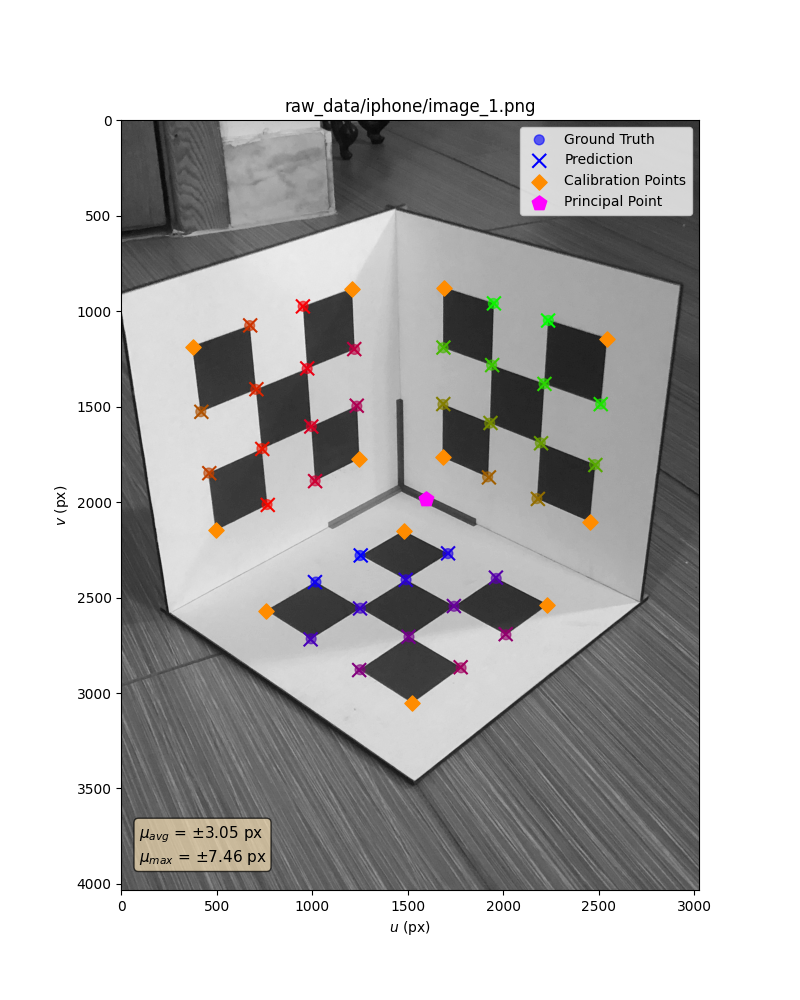
\includegraphics[width=0.6\textwidth]{assets/graphs/iphone_graph}
    \caption{Graph produced by \texttt{Matplotlib} which displays the results of the trial}
\end{figure}

\begin{equation*}
    P =
    \begin{bmatrix}
        \num{-2.5844e-03} & \num{1.7334e-03}  & \num{-4.6719e-04} & \num{6.0581e-01} \\
        \num{4.8240e-04}  & \num{4.4097e-04}  & \num{-3.1337e-03} & \num{7.9559e-01} \\
        \num{-3.3990e-07} & \num{-3.1311e-07} & \num{-2.8179e-07} & \num{4.1340e-04}
    \end{bmatrix}
\end{equation*}

\begin{table}[H]
    \centering
    \caption{Parameters}
    \begin{tabular}{| C{0.15\textwidth} | C{0.30\textwidth} |}
        \hline
        Parameter & Value                   \\
        \hline
        \hline
        $f_x$     & $\qty{5590.3}{\pixel}$ \\
        $f_y$     & $\qty{5571.7}{\pixel}$ \\
        \hline
        $c_x$     & $\qty{1595.2}{\pixel}$ \\
        $c_y$     & $\qty{1983.1}{\pixel}$ \\
        \hline
        $\alpha$  & $\qty{38.90}{\degree}$  \\
        $\beta$   & $\qty{29.52}{\degree}$  \\
        $\gamma$  & $\qty{-48.01}{\degree}$ \\
        \hline
        $t_x$     & $\qty{470.7}{\mm}$     \\
        $t_y$     & $\qty{457.6}{\mm}$     \\
        $t_z$     & $\qty{390.7}{\mm}$     \\
        \hline
    \end{tabular}
\end{table}


The reprojection error, $\mu$, was calculated to be $\pm \qty{3.02}{\pixel}$.


\section{Conclusion}
From my rudimentary experimental validation, we can see that my devised method of camera calibration is very accurate, and despite its various limitations, such as fixed focal length and fixed locality, it serves as a proof of concept which excellently demonstrates the fundamental techniques behind camera calibration.

% ================================================================

%TC:ignore
\section*{Acknowledgements}
\addcontentsline{toc}{section}{Acknowledgements}

I am very grateful to my supervisor Mr. Hoteit for his continual guidance and invaluable pieces of advice during the process of writing this extended essay. Additionally, I would like to express my appreciation to Mr. Auclair for dedicating his time to instruct me on camera operation and familiarizing me with camera settings. I am also indebted to Mr. Matthewson for his guidance with the manufacturing of my calibration object, and to Leon, for his help in operating the laser cutter. Last but not least, I want to thank Aditya for aiding me in the process of creating some of the diagrams used in my paper.
\clearpage
\pagestyle{backmatter}

\printbibliography[heading=bibintoc]{}

% =================================================================

\clearpage
\begin{appendices}
    \pagestyle{appendices}
    \section{Calibration Object Details}
\subsection{Panels}
\subsection{Grid Pattern}

\begin{center}
    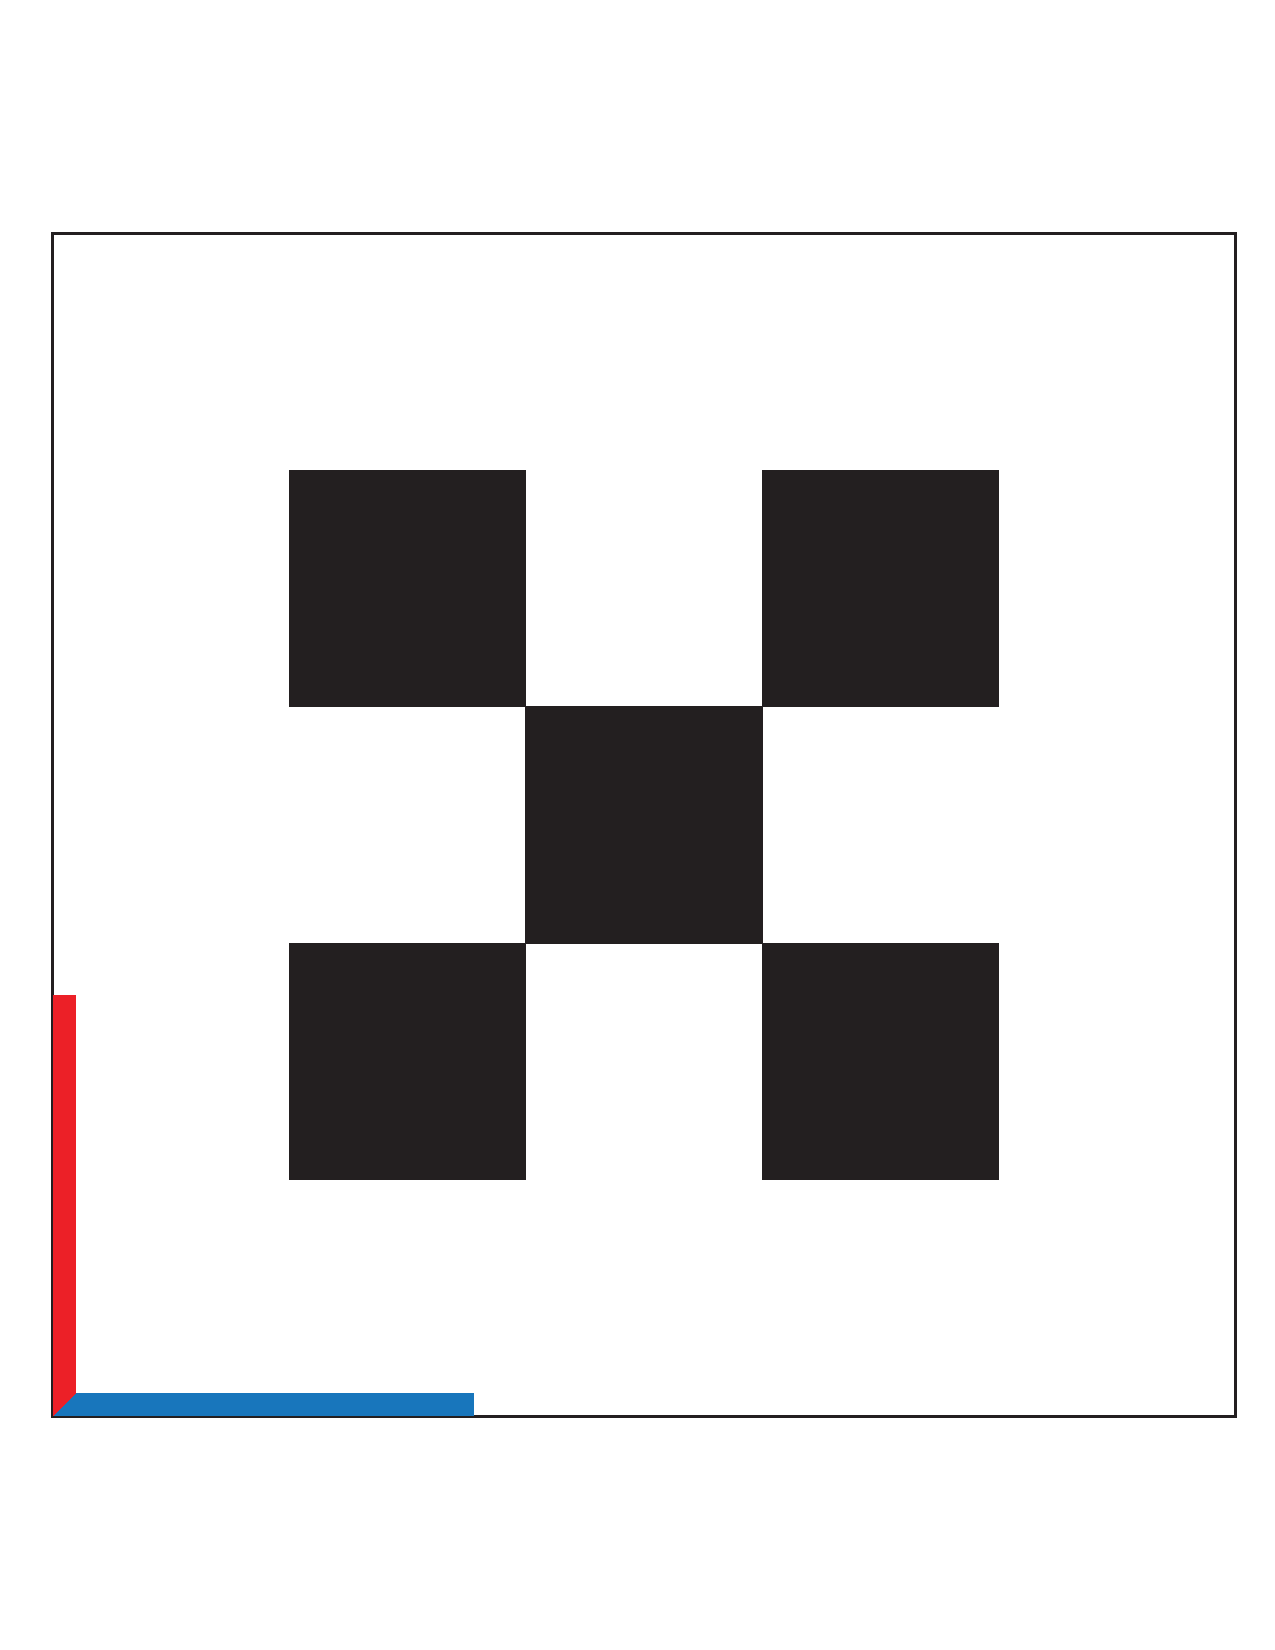
\includepdf[pages={1-}]{grid.pdf}
\end{center}


    \section{Source Code}

\subsection*{Project Structure}

\dirtree{%
    .1 calicam.
    .2 calicam.
    .3 \_\_init\_\_.py.
    .3 \hyperref[code:extract]{extract.py}.
    .3 \hyperref[code:parser]{parser.py}.
    .3 \hyperref[code:projection]{projection.py}.
    .3 \hyperref[code:vecs]{vecs.py}.
    .2 \hyperref[code:run]{run.py}.
}

\subsubsection*{run.py} \label{code:run}
\inputminted{python}{./calicam/run.py}

\subsubsection*{calicam/parser.py} \label{code:parser}
\inputminted{python}{./calicam/calicam/parser.py}

\subsubsection*{calicam/projection.py} \label{code:projection}
\inputminted{python}{./calicam/calicam/projection.py}

\subsubsection*{calicam/extract.py} \label{code:extract}
\inputminted{python}{./calicam/calicam/extract.py}

\subsubsection*{calicam/vecs.py} \label{code:vecsZ}
\inputminted{python}{./calicam/calicam/vecs.py}

\end{appendices}
%TC:endignore

\end{document} % END

